\documentclass[11pt]{article}
\usepackage[a4paper,margin=1in]{geometry}
\usepackage[T1]{fontenc}
\usepackage[utf8]{inputenc}
\usepackage{lmodern,microtype,amsmath,amssymb,graphicx,booktabs,array,longtable,placeins}
\usepackage{setspace,float,pdflscape}
\usepackage[style=apa,natbib=true,backend=biber,sortcites=true,sorting=nyt]{biblatex}
\addbibresource{../06_Bibliography/aeri_refs.bib}
\usepackage[colorlinks=true,citecolor=blue,linkcolor=blue,urlcolor=black]{hyperref}
\usepackage{caption}
\captionsetup{font=small,labelfont=bf}
\graphicspath{{Supplementary_Data/Figures/}}
\onehalfspacing
\setlength{\emergencystretch}{2em}
\title{Online Supplement to\\[4pt]\textit{Measuring Economic Risk in Africa: The African Economic Risk Index and African Risk Score}}
\author{}
\date{September 2026}
\begin{document}
\renewcommand{\thetable}{S\arabic{table}}
\renewcommand{\thefigure}{S\arabic{figure}}
\renewcommand{\theequation}{S\arabic{equation}}
\begin{center}
{\Large\bfseries Supplementary Material to\\[4pt]\textit{Measuring Economic Risk in Africa: The African Economic Risk Index and African Risk Score}\par}
\vspace{.35cm}September 2026
\end{center}
\begin{abstract}\singlespacing
This supplement provides material that supports the measurement and empirical results reported in the paper without interrupting its main argument. It records the domain definitions used for the eight risk pillars, the PCA conversion used for the bounded composite measures, detailed PVAR estimation and inference, expanded exact-text deduplication results, additional external-identification results, and country-level AERI and ARS outputs. The supplement uses the same analytical vintage and definitions as the paper.
\end{abstract}
\tableofcontents
\clearpage

\section{Detailed Pillar Descriptions}
The main paper condenses the eight pillar descriptions. The definitions below record the domain interpretation used in the analytical vintage. Pillars are non-exclusive: one article can contribute to several domains when its economic content spans them.

\subsection{Inflation Risk}
Inflation-related reporting covers price pressures and their implications for households and firms. Its mean pillar index is 4.34 points across eligible country-months. Sustained increases can reflect greater attention to input costs, purchasing power, administered prices or anticipated price adjustment. The positive and persistent response of headline inflation to an inflation-risk innovation in the paper provides an external check on this interpretation.

\subsection{FX and External Risk}
External-risk reporting covers exchange-rate conditions, foreign-currency availability and external financing. Its mean pillar index is 5.03 points. Currency conditions affect imported-input costs and access to external finance, so overlap with inflation and financial-sector reporting is economically natural. The reverse-response evidence in the paper also shows that realised depreciation is followed by a higher aggregate AERI reading.

\subsection{Debt and Fiscal Risk}
Fiscal reporting covers public borrowing, debt service, revenue pressure and constraints on government finances. Its mean pillar index is 8.64 points. Fiscal concerns often coincide with financial-sector pressure when public financing conditions affect domestic intermediaries and with external risk when foreign-currency obligations become more salient. The overlapping classification preserves those connections within the news record.

\subsection{Financial-Sector Risk}
Financial-sector reporting covers intermediation, liquidity, balance-sheet pressure and financial stability. Its mean pillar index is 11.46 points, the largest pooled pillar mean in this vintage. The level describes the prominence of financial-sector concerns in the retained corpus and is interpreted together with within-pillar changes over time.

\subsection{Growth and Real-Economy Risk}
Real-economy reporting covers production, employment, demand and broader economic activity. Its mean pillar index is 3.17 points. News can register weakening demand or production constraints before a complete statistical account becomes available and can also respond to realised changes in activity. The reverse-response analysis in the paper shows how the aggregate AERI responds to a monthly GDP-growth innovation.

\subsection{Commodity and Supply Risk}
Commodity and supply reporting covers resource production, logistics and disruptions to supply. Its mean pillar index is 0.09 points. The low pooled mean reflects the concentration of such reporting in particular countries and episodes. For interpretation, changes within exposed economies are more informative than the continental average alone.

\subsection{Political-Economy Risk}
Political-economy reporting covers governance, policy implementation and their economic consequences. Its mean pillar index is 4.94 points. Political content enters the framework when it carries economic relevance and scored risk content, allowing governance and implementation concerns to be identified within broader high-risk episodes.

\subsection{Climate and Disaster Risk}
Climate and disaster reporting covers environmental disruptions and their economic effects. Its mean pillar index is 1.25 points. Such events are geographically concentrated and irregular, so the pillar is most useful as a domain-specific diagnostic read alongside country context and event data.

\section{Formal PCA Conversion and Aggregation Details}
Let $X_j$ denote a bounded input, with calibration mean $\mu_j$, standard deviation $s_j$ and oriented first-component loading $v_j$. For standardized inputs $Z_j=(X_j-\mu_j)/s_j$,
\begin{equation}
 v'Z=\sum_j \frac{v_j}{s_j}X_j-\sum_j\frac{v_j\mu_j}{s_j}.
\end{equation}
Define $D=\sum_j v_j/s_j>0$ and $w_j=(v_j/s_j)/D$. Then
\begin{equation}
100\sum_jw_jX_j=\frac{100}{D}\left(v'Z+\sum_j\frac{v_j\mu_j}{s_j}\right).
\end{equation}
The bounded-input score is therefore an affine rescaling of the first principal component. The implementation rejects calibration standard deviations below $10^{-10}$ and materially negative oriented loadings below $-10^{-9}$; negligible numerical negatives are set to zero before normalization. Calculations use the unrounded weights reported in the project outputs.

Annual AERI and raw pillar indices weight monthly values by retained article counts so that annual numerators and denominators correspond to the same article universe. Annual breadth is the ratio of summed relevant articles to summed retained articles, while annual severity weights monthly conditional severity by relevant-article counts. When annual ARS or the eight-pillar PCA composite is required, the nonlinear composite is recomputed from annual inputs rather than formed as an average of monthly composite scores.

\section{Detailed PVAR Specification and Inference}\label{app:pvar}
\subsection{Macroeconomic Data and Pooled Panel Estimation}\label{sec:pooled_method}
The empirical assessment relates monthly news-based risk to headline inflation, exchange-rate depreciation and monthly GDP growth. Its purpose is to test whether the measured domains display economically interpretable dynamics. ARS calibration is completed independently of these macroeconomic outcomes, preserving a clean separation between index construction and subsequent validation.

\subsubsection{Monthly variables and sample construction}
Headline inflation, $\pi_{ct}$, is the supplied monthly observation of the inflation rate. The exchange rate, $e_{ct}$, is expressed as local-currency units per US dollar. Monthly GDP, $G_{ct}$, is the supplied purchasing-power-parity GDP series. Depreciation and monthly GDP growth are defined as
\begin{equation}
 d_{ct}=100[\log e_{ct}-\log e_{c,t-1}],\qquad
 g_{ct}=100[\log G_{ct}-\log G_{c,t-1}].\label{eq:macro_growth}
\end{equation}
Thus a positive $d_{ct}$ denotes depreciation, whereas a positive $g_{ct}$ denotes monthly GDP growth. Headline inflation retains the definition supplied in the macroeconomic panel, while depreciation and GDP growth are the log-difference transformations above. The sample-specific winsorisation bounds are reported below.

The main validation specification uses one news-based risk measure at a time---the inflation-risk pillar, the FX and external-risk pillar, AERI or ARS---together with inflation, depreciation and monthly GDP growth. The estimation sample is distinct from the descriptive sample defined by the 100-article threshold. It begins with the 36-country union selected by the prior correlation screen, then retains country-months with the risk measure, the required macroeconomic inputs and the full lag structure, subject to at least 24 usable observations per country.\footnote{The estimation panel winsorises the supplied macroeconomic transformations at pooled first and ninety-ninth percentiles. In the GDP-augmented sample the retained bounds are $[-2.565,50.934]$ for inflation, $[-5.736,14.926]$ for depreciation and $[-0.819,1.506]$ for monthly GDP growth.} The common GDP-augmented panel contains 4,286 observations for 36 countries and runs from May 2015 to December 2025. The 100-article rule continues to govern the principal descriptive country comparisons and ARS calibration; it is not imposed on the PVAR estimation panel. This distinction explains why a country can appear in the PVAR sample even when few or no months satisfy the descriptive coverage threshold. Using the direct pillar indices in this specification keeps the economic interpretation aligned with the measurement framework in the main text. Supporting transformations and country-level estimation diagnostics are available from the authors on request.

Risk innovations are put on a comparable within-country scale. Let $\bar r_c$ be the country mean in the supplied scaling panel and $s_{r,w}$ the sample standard deviation of $r_{ct}-\bar r_c$ pooled across that panel. We use $\widetilde r_{ct}=r_{ct}/s_{r,w}$; country effects subsequently absorb level differences. A one-unit risk innovation therefore represents one pooled within-country standard deviation, rather than one raw index point. Scaling parameters are fixed for the reported estimates and bootstrap exercises.

\subsubsection{The pooled dynamic system}
For $m$ endogenous variables, the maintained model is
\begin{equation}
 y_{ct}=\alpha_c+\lambda_t+\sum_{\ell=1}^{p}B_\ell y_{c,t-\ell}+\varepsilon_{ct},\qquad
 E(\varepsilon_{ct}\varepsilon_{ct}')=\Sigma.\label{eq:pvar}
\end{equation}
Here $\alpha_c$ captures persistent country differences, and $\lambda_t$ is a full year-month effect that absorbs shocks common to countries in a given month. The year-month effects therefore absorb common calendar-time variation rather than recurring month-of-year seasonality alone. The slope matrices $B_\ell$ are pooled across countries. In the three-variable system, $y_{ct}=(\widetilde r_{ct},\pi_{ct},d_{ct})'$. In the GDP-augmented system, $y_{ct}=(\widetilde r_{ct},\pi_{ct},d_{ct},g_{ct})'$. In particular, the inflation equation in the latter system is
\begin{align}
 \pi_{ct}={}&\alpha_c^\pi+\lambda_t^\pi+
 \sum_{\ell=1}^{p}\bigl(b_{\pi r,\ell}\widetilde r_{c,t-\ell}
 +b_{\pi\pi,\ell}\pi_{c,t-\ell}\notag\\
 &\hspace{35mm}+b_{\pi d,\ell}d_{c,t-\ell}
 +b_{\pi g,\ell}g_{c,t-\ell}\bigr)+\varepsilon_{ct}^\pi.\label{eq:inflation_equation}
\end{align}
The risk, depreciation and GDP equations have the same lag structure with equation-specific coefficients. Each outcome can therefore respond to its own history and to the histories of the other variables. Pooling provides a common dynamic description conditional on fixed effects. The multivariate panel structure follows the empirical framework in \citet{love2006} and \citet{abrigo2016}, implemented here with within-transformed pooled least squares.

Let $X$ stack all $mp$ lagged regressors and $Y$ stack the contemporaneous outcomes on the common estimation sample. Alternating country and year-month projections yield $\ddot X$ and $\ddot Y$. The pooled estimator and residual covariance are
\begin{equation}
 \widehat B=(\ddot X'\ddot X)^+\ddot X'\ddot Y,\quad
 \widehat E=\ddot Y-\ddot X\widehat B,\quad
 \widehat\Sigma=\frac{\widehat E'\widehat E}{n-mp}.\label{eq:pooled_ols}
\end{equation}
The superscript $+$ denotes the Moore--Penrose inverse; the covariance denominator is the implemented lag-regressor adjustment. A common maximum-lag sample is used when comparing candidate orders, preventing changes in the available observations from driving lag choice. Among stable candidates with $p\in\{1,2,3\}$, the criterion is
\begin{equation}
 \mathrm{BIC}(p)=\log|\widehat\Sigma_p|+\frac{\log n}{n}m^2p.\label{eq:bic}
\end{equation}
Stability requires the maximum absolute companion-matrix eigenvalue to lie below the numerical threshold of 0.999. All reported specifications select three lags. Table~\ref{tab:model_diagnostics} reports observations, country counts, roots and accepted bootstrap draws. Fixed-effects estimation with lagged outcomes can retain finite-time bias \citep{nickell1981}; the long monthly dimension reduces some finite-sample concerns but leaves this source of bias relevant to interpretation.

\subsubsection{Identification and impulse responses}
Let $\widehat\Sigma=LL'$ with $L$ lower triangular. Forward systems order risk first, followed by inflation, depreciation and monthly GDP growth where included. This permits a risk innovation to affect the macroeconomic variables within the month, while assigning contemporaneous feedback into risk to subsequent periods. For reverse responses, the order is inflation, depreciation, monthly GDP growth and AERI. The two orderings answer complementary recursive questions about forward risk propagation and macroeconomic feedback.

The moving-average matrices and normalised responses are
\begin{align}
 \Phi_0&=I_m,\qquad
 \Phi_h=\sum_{\ell=1}^{\min(p,h)}\widehat B_\ell\Phi_{h-\ell},\label{eq:ma}\\
 \theta_{kj}(h)&=\frac{e_k'\Phi_hLe_j}{e_j'Le_j},\qquad h=0,\ldots,12,\label{eq:irf}
\end{align}
where $e_j$ is the $j$th coordinate vector, distinct from the exchange-rate notation in equation~\eqref{eq:macro_growth}. The denominator normalises the innovation to a one-unit contemporaneous increase in the selected variable. For forward risk innovations, that unit is one within-country standard deviation. For reverse macroeconomic innovations, it is one percentage point. This convention makes the reported response magnitudes explicit while preserving the natural units used for the macroeconomic innovations.

\subsubsection{Inference and interpretation}
Uncertainty bands are constructed by resampling countries with replacement, retaining each selected country's complete time history, and re-estimating the fixed-effects system. The lag order, measurement transformations and fixed ARS calibration remain unchanged across bootstrap replications. Four hundred accepted stable replications provide the fifth and ninety-fifth percentiles at each horizon. These are pointwise 90 percent intervals, so each band describes uncertainty at a given horizon. Simultaneous inference for the full response path or for the location of its population peak would require a different procedure.

Joint lag tests complement the IRFs. For example, the inflation equation tests
\begin{equation}
 H_0:b_{\pi r,1}=\cdots=b_{\pi r,p}=0,\qquad
 W=(R\widehat\beta)'[R\widehat V R']^+(R\widehat\beta),\label{eq:wald}
\end{equation}
using country-cluster covariance $\widehat V$ and a $\chi_p^2$ reference distribution. The exact covariance calculation is given in Appendix~\ref{app:pvar}. Rejection indicates incremental information in the included lagged variable conditional on the other lags and fixed effects. The recursive response additionally reflects contemporaneous residual covariance and propagation through the full system, so the tables report both forms of evidence.


\begin{table}[htbp]\centering\small\singlespacing
\caption{Pooled PVAR samples and stability diagnostics}\label{tab:model_diagnostics}
\setlength{\tabcolsep}{4pt}
\begin{tabular}{lrrrrrr}\toprule
System & Variables & Countries & Obs. & Lags & Max. root & Draws\\\midrule
Inflation risk + GDP & 4 & 36 & 4,286 & 3 & 0.9228 & 400/400\\
FX/external risk + GDP & 4 & 36 & 4,286 & 3 & 0.9222 & 400/400\\
AERI + GDP & 4 & 36 & 4,286 & 3 & 0.9198 & 400/400\\
ARS + GDP & 4 & 36 & 4,286 & 3 & 0.9190 & 400/400\\
\bottomrule\end{tabular}
\par\medskip\raggedright\footnotesize\textit{Notes:} All samples span May 2015--December 2025 and use the same 36-country correlation-selected panel. The PVAR sample is formed from complete model inputs and lags with at least 24 usable observations per country; the 100-article rule used for descriptive country comparisons is not imposed here. Draws report accepted/attempted country-cluster replications. A companion root below one indicates fitted dynamic stability; identification is assessed separately through the stated recursive and external-shock designs.
\end{table}

The 36-country set is the inclusive union of countries whose earlier country-level screening exercise produced an absolute correlation of at least 0.30 for either inflation-risk versus inflation or FX/external-risk versus the exchange rate. Twenty-eight countries enter through the inflation screen, fourteen through the exchange-rate screen and six through both. The set comprises Algeria, Angola, Botswana, Burkina Faso, Burundi, Cameroon, Cape Verde, Comoros, Democratic Republic of the Congo, Egypt, Ethiopia, Gambia, Ghana, Guinea, Guinea-Bissau, Ivory Coast, Lesotho, Liberia, Libya, Malawi, Mali, Mauritius, Morocco, Mozambique, Namibia, Nigeria, Sao Tome and Principe, Senegal, Sierra Leone, Somalia, South Africa, Tanzania, Tunisia, Uganda, Zambia and Zimbabwe.

The PVAR estimation sample should be read separately from the descriptive coverage sample reported later in this supplement. AERI and the pillar series are available for lower-volume country-months, whereas the 100-article threshold is used to define the principal descriptive comparisons and the ARS calibration sample. The PVAR retains the correlation-selected countries with complete model inputs and the required lag structure and imposes a minimum of 24 usable observations per country. This is why Guinea-Bissau and Sao Tome and Principe can enter the PVAR even though Table~\ref{tab:all_country_aeri_ars} reports zero and twenty months, respectively, under the stricter 100-article descriptive rule.

For equation $k$, write the country-cluster score as $s_{ck}=\ddot X_c'\widehat\varepsilon_{ck}$, let $q=mp$, and denote the number of countries by $C$. The covariance used in the joint lag tests is
\begin{equation}
\widehat V_k=
\frac{C}{C-1}\frac{n-1}{n-q}
(\ddot X'\ddot X)^+
\left(\sum_{c=1}^{C}s_{ck}s_{ck}'\right)
(\ddot X'\ddot X)^+.
\end{equation}
Country resampling preserves dependence within each country's observed history. Year-month effects absorb common calendar-time variation. Inference is conditional on the correlation-screened country set and on the fixed ARS calibration.

\section{Exact-Text Deduplication: Expanded Results}
Repeated publication can alter a country-month index when identical high-scoring text appears in several records. The robustness exercise decodes article bodies, restricts comparison to bodies of at least 200 characters, and collapses exact matches within each country-month. Appearances in different countries or different months remain separate observations. Edited stories, translations and rewritten versions also remain separate because the test is deliberately exact.

The reconstruction covers 21,303,020 frozen-vintage records in 7,126 country-months. It is 553 records and one Togo country-month short of the archived aggregate because 42 source files were empty or unreadable. Where a reconstructed month does not fully match the archived count, unmatched frozen-vintage records remain in the denominator and only directly observed duplicates are removed. This preserves the archived universe while allowing the contribution of verified repetitions to be measured.

\begin{table}[htbp]\centering\small
\caption{Sensitivity to within-country-month exact-text deduplication}\label{tab:deduplication}
\begin{tabular}{@{}lr@{}}\toprule Statistic & Result \\\midrule
Records removed & 497,091 \\
Removed share (percent) & 2.33 \\
Cross-outlet copies removed & 186,379 \\
AERI Pearson correlation & 0.9296 \\
AERI rank correlation & 0.9883 \\
AERI mean absolute change & 2.32 \\
AERI 95th-percentile absolute change & 8.30 \\
ARS Pearson correlation & 0.9680 \\
ARS mean absolute change & 0.61 \\
Months falling below 100 articles & 69 \\
\bottomrule\end{tabular}
\begin{singlespace}\footnotesize\textit{Notes:} The comparison uses 6,418 country-months with at least 100 articles before and after deduplication. Exact duplicates have the same decoded body within a country-month; bodies shorter than 200 characters are retained. Both numerator and denominator are adjusted. ARS uses the original unrounded PCA weights.\end{singlespace}\end{table}

Figure~\ref{fig:supp_dedup} compares the monthly cross-country median AERI before and after exact-text removal on the common coverage sample. The two paths retain the same broad chronology and both peak in April 2020. The differences are concentrated in particular countries and months rather than spread evenly through the panel.

\begin{figure}[htbp]\centering
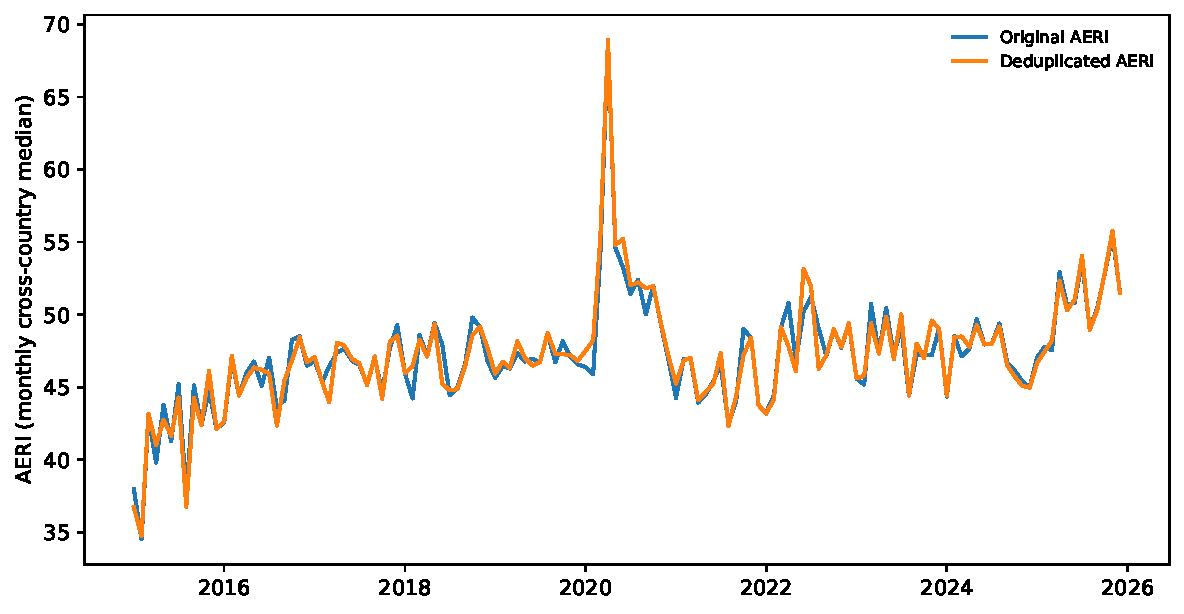
\includegraphics[width=.92\textwidth]{Supplement_Figure_S1.pdf}
\caption{Monthly median AERI before and after within-country-month exact-text deduplication}
\label{fig:supp_dedup}
\begin{singlespace}\footnotesize\textit{Notes:} Each line is the cross-country median among country-months in the common coverage sample used for the deduplication comparison. The aggregate peak remains April 2020.\end{singlespace}
\end{figure}

\begin{table}[htbp]\centering\scriptsize\setlength{\tabcolsep}{4pt}
\caption{Country-level sensitivity of AERI peaks to exact-text deduplication}\label{tab:supp_dedup_country}
\begin{tabular}{lrrrrl}\toprule
Country & Original & Dedup. at original & $\Delta$ & Within-country $r$ & Dedup. peak\\\midrule
Sierra Leone & 269.72 & 110.77 & -158.95 & 0.812 & 2016-10\\
Rwanda & 95.43 & 63.35 & -32.08 & 0.984 & 2020-04\\
Mauritius & 91.64 & 111.79 & 20.15 & 0.998 & 2020-05\\
Angola & 85.67 & 72.69 & -12.98 & 0.932 & 2020-04\\
Eswatini & 75.11 & 87.01 & 11.89 & 0.908 & 2020-04\\
Zambia & 121.49 & 130.62 & 9.12 & 0.684 & 2024-09\\
Cameroon & 68.83 & 60.92 & -7.91 & 0.992 & 2016-12\\
Botswana & 90.44 & 85.72 & -4.72 & 0.972 & 2025-12\\
\bottomrule\end{tabular}
\begin{singlespace}\footnotesize\textit{Notes:} Countries shown are those with the largest absolute change at the original peak, augmented to retain Rwanda and Mauritius because their peak behavior is discussed in the paper. The correlation is computed over the common within-country monthly sample. A change can be positive because removing duplicate records changes both the score numerator and the all-article denominator.\end{singlespace}
\end{table}

The median within-country AERI correlation is 0.9992 and 48 of 53 countries retain the same peak month on the common sample. Sierra Leone is the largest exception: its November 2016 observation falls from 269.72 to 110.77 and the deduplicated peak moves to October 2016. Rwanda's August 2021 observation falls from 95.43 to 63.35, while Mauritius rises from 91.64 to 111.79 in May 2020 because removal changes both the numerator and denominator. These cases identify where syndicated or repeated identical text materially affects a country history while leaving the continental chronology largely unchanged.

\section{External Monetary-Policy Exposure: Additional Results}
The external-identification exercise uses the pure U.S. monetary-policy surprise from \citet{jarocinski2020}, aggregated to the month and standardized over the 2015--2025 sample. Predetermined exposure is the 2014 stock of external debt as a share of GNI from the World Bank, transformed as $\log(1+x)$ and standardized. For country $i$ and horizon $h$, the preferred local projection is
\begin{align}
\mathrm{AERI}_{i,t+h}-\mathrm{AERI}_{i,t-1}
={}&\alpha_i^h+\gamma_t^h+\beta_h(MP_t\times E_i^{2014})\notag\\
&+\sum_{\ell=1}^{3}\theta_{h\ell}\Delta\mathrm{AERI}_{i,t-\ell}
+\sum_{\ell=1}^{3}\psi_{h\ell}(MP_{t-\ell}\times E_i^{2014})
+\varepsilon_{i,t+h}.
\end{align}
Country effects absorb persistent differences in average AERI and year-month effects absorb shocks shared by the African sample in a given month. The identifying variation is the cross-country difference in predetermined exposure to the same externally measured tightening. Standard errors are two-way clustered by country and month, and finite-cluster inference uses 28 denominator degrees of freedom for the 29-country cross-section.

\begin{figure}[htbp]\centering
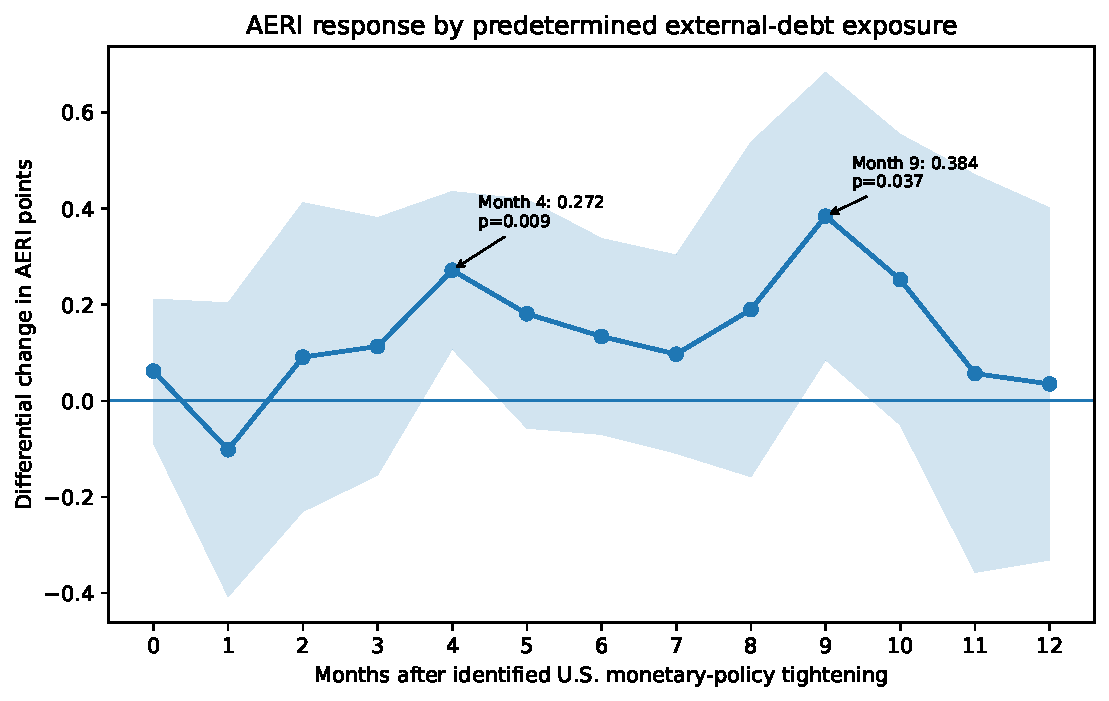
\includegraphics[width=.88\textwidth]{Supplement_Figure_S2.pdf}
\caption{Differential AERI response to an externally identified U.S. monetary-policy tightening}
\begin{singlespace}\footnotesize\textit{Notes:} The line reports $\widehat\beta_h$. Shading gives pointwise 90 percent finite-cluster intervals. Exposure is standardized $\log(1+\text{2014 external debt/GNI})$.\end{singlespace}
\end{figure}

\begin{table}[htbp]\centering\small
\caption{Full horizon path for the external monetary-policy exposure specification}\label{tab:supp_external_horizons}
\begin{tabular}{rrrrr}\toprule
Horizon & $\hat\beta_h$ & 90\% CI lower & 90\% CI upper & $p$-value\\\midrule
0 & 0.062 & -0.088 & 0.212 & 0.487\\
1 & -0.102 & -0.407 & 0.204 & 0.576\\
2 & 0.091 & -0.230 & 0.412 & 0.633\\
3 & 0.113 & -0.155 & 0.381 & 0.478\\
4 & 0.272 & 0.108 & 0.436 & 0.009\\
5 & 0.181 & -0.057 & 0.419 & 0.206\\
6 & 0.134 & -0.070 & 0.338 & 0.273\\
7 & 0.097 & -0.109 & 0.304 & 0.430\\
8 & 0.190 & -0.158 & 0.538 & 0.360\\
9 & 0.384 & 0.085 & 0.684 & 0.037\\
10 & 0.252 & -0.050 & 0.554 & 0.167\\
11 & 0.057 & -0.357 & 0.471 & 0.817\\
12 & 0.035 & -0.331 & 0.402 & 0.871\\
\bottomrule\end{tabular}
\begin{singlespace}\footnotesize\textit{Notes:} The coefficient is the differential cumulative AERI response to a one-standard-deviation U.S. monetary-policy tightening for a country one standard deviation higher in predetermined 2014 external-debt exposure. Intervals and $p$-values use the finite-cluster reference with 28 denominator degrees of freedom.\end{singlespace}
\end{table}
\begin{table}[htbp]\centering
\caption{Externally identified monetary-policy exposure validation}
\label{tab:external_identification}
\begin{singlespace}\scriptsize
\setlength{\tabcolsep}{3pt}
\begin{tabular}{@{}p{4.7cm}cccc@{}}
\toprule
Specification & $\hat\beta_4$ & $p_4$ & $\hat\beta_9$ & $p_9$\\
\midrule
Primary: log debt/GNI & 0.272 & 0.0086 & 0.384 & 0.0373\\
Raw debt/GNI & 0.203 & 0.0152 & 0.289 & 0.0556\\
95th-percentile-capped debt/GNI & 0.230 & 0.0284 & 0.347 & 0.0566\\
Exclude Mozambique & 0.265 & 0.0305 & 0.390 & 0.0610\\
African-country panel restricted to FOMC announcement months & 0.299 & 0.0078 & 0.354 & 0.0395\\
Alternative monetary-policy shock & 0.251 & 0.0068 & 0.420 & 0.0534\\
\midrule
Leave-one-country-out range & [0.214, 0.308] & 29/29 $p<0.10$ & [0.282, 0.455] & 29/29 $p<0.10$\\
\bottomrule
\end{tabular}
\end{singlespace}
\begin{singlespace}\footnotesize\textit{Notes:} The dependent variable is the cumulative change in AERI from month $t-1$ through horizon $h$. The shock is the standardized pure U.S. monetary-policy surprise from the Jaroci\'{n}ski--Karadi high-frequency decomposition, aggregated to the month. Predetermined exposure is 2014 external debt stocks as a share of GNI from the World Bank, transformed as $\log(1+x)$ and standardized in the primary specification. All regressions include country and year-month fixed effects, three lags of the AERI change and three lags of the shock--exposure interaction. Standard errors are two-way clustered by country and month. Reported $p$-values use a finite-cluster $t$ reference with degrees of freedom equal to the number of African-country clusters minus one. Restricted wild-cluster-bootstrap $p$-values for the primary month-four and month-nine coefficients are 0.042 and 0.034, respectively. In the leave-one-country-out exercise, 28 of 29 month-four estimates and 24 of 29 month-nine estimates also satisfy $p<0.05$.\end{singlespace}
\end{table}

\begin{table}[htbp]\centering
\caption{External-identification diagnostics and falsification checks}
\label{tab:external_id_diagnostics}
\begin{singlespace}\scriptsize
\setlength{\tabcolsep}{3pt}
\begin{tabular}{@{}p{4.5cm}p{3.4cm}p{4.8cm}@{}}
\toprule
Check & Statistic / range & Interpretation\\
\midrule
Pre-shock AERI-change placebos (1--6 months) & $p\in[0.156,0.807]$ & None significant at 10 percent\\
CBI shock $\times$ exposure, month 4 & $p=0.153$ & p-value above 0.10\\
CBI shock $\times$ exposure, month 9 & $p=0.125$ & p-value above 0.10\\
Joint future-shock interaction placebo & $\chi^2(6)=11.30$, asymptotic $p=0.079$ & Large-sample reference only\\
Finite-cluster joint reference & $F(6,28)=1.884$, $p=0.119$ & p-value above 0.10\\
Restricted wild-cluster bootstrap & $p=0.221$ & p-value above 0.10\\
\bottomrule
\end{tabular}
\end{singlespace}
\begin{singlespace}\footnotesize\textit{Notes:} The joint future-shock placebo includes the contemporaneous monetary-policy-shock--exposure interaction as a control. The asymptotic Wald reference is reported for transparency, but the preferred joint inference recognizes that the identifying cross-section contains 29 African-country clusters. The finite-cluster $F$ reference uses 28 denominator degrees of freedom; the restricted wild-cluster bootstrap uses 999 Rademacher replications by African country. The pre-shock outcome placebos are estimated without lagged dependent-variable controls that would mechanically span the placebo outcome.\end{singlespace}
\end{table}


The horizon path is delayed. The differential response reaches 0.272 AERI points at month four, with a 90 percent interval of $[0.108,0.436]$, and 0.384 points at month nine, with interval $[0.085,0.684]$. The six reported robustness variants retain positive month-four and month-nine coefficients. Leave-one-country-out estimates remain positive across all 29 omissions. Pre-shock outcomes and the central-bank-information component of the same announcements do not reproduce the exposure pattern, while the finite-cluster and restricted wild-cluster references place the joint future-shock placebo above conventional significance thresholds. Complete monthly shock, exposure and intermediate estimation files are available from the authors on request.

\section{All-Country AERI and ARS Outputs}
Table~\ref{tab:all_country_aeri_ars} reports compact AERI and ARS outputs for all 54 economies in the 2015--2025 panel. The month count refers only to country-months with at least 100 retained articles. It is therefore a descriptive-coverage statistic rather than a PVAR eligibility count.

\begin{landscape}
\setlength{\tabcolsep}{3pt}\begin{longtable}{lrrrlrrl}
\caption{Country-level AERI and ARS summary statistics, 2015--2025}\label{tab:all_country_aeri_ars}\\
\toprule
Country & Months & Mean AERI & Max AERI & AERI peak & Mean ARS & Max ARS & ARS peak\\
\midrule
\endfirsthead
\multicolumn{8}{c}{\tablename\ \thetable{} -- continued from previous page}\\
\toprule
Country & Months & Mean AERI & Max AERI & AERI peak & Mean ARS & Max ARS & ARS peak\\
\midrule
\endhead
\midrule \multicolumn{8}{r}{Continued on next page}\\ \endfoot
\bottomrule \endlastfoot
Algeria & 132 & 65.02 & 83.44 & 2020-04 & 44.67 & 50.57 & 2020-04\\
Angola & 132 & 53.45 & 85.67 & 2019-10 & 39.45 & 49.07 & 2020-05\\
Benin & 132 & 43.38 & 71.98 & 2020-04 & 36.28 & 45.65 & 2020-04\\
Botswana & 132 & 69.39 & 90.44 & 2025-12 & 43.67 & 49.59 & 2025-12\\
Burkina Faso & 132 & 47.73 & 68.40 & 2020-04 & 37.90 & 46.83 & 2020-04\\
Burundi & 132 & 49.20 & 84.80 & 2022-08 & 37.84 & 49.40 & 2022-08\\
Cameroon & 132 & 48.06 & 68.83 & 2018-11 & 38.77 & 46.58 & 2018-11\\
Cape Verde & 131 & 39.73 & 67.21 & 2022-07 & 31.79 & 42.38 & 2022-06\\
Central African Republic & 129 & 62.25 & 116.38 & 2017-04 & 39.97 & 53.18 & 2017-04\\
Chad & 96 & 55.64 & 103.13 & 2020-04 & 38.72 & 54.16 & 2020-04\\
Comoros & 130 & 42.83 & 73.75 & 2022-06 & 36.58 & 47.39 & 2025-02\\
Republic of the Congo & 132 & 61.63 & 87.31 & 2020-05 & 41.42 & 48.92 & 2020-05\\
Democratic Republic of the Congo & 132 & 55.00 & 85.25 & 2020-08 & 38.92 & 48.42 & 2022-04\\
Djibouti & 4 & 64.96 & 73.62 & 2024-05 & 41.17 & 45.06 & 2024-05\\
Egypt & 132 & 40.55 & 97.11 & 2025-12 & 35.94 & 51.26 & 2025-12\\
Equatorial Guinea & 73 & 21.10 & 45.64 & 2020-05 & 18.78 & 28.19 & 2020-05\\
Eritrea & 132 & 49.29 & 77.55 & 2024-06 & 37.40 & 46.61 & 2021-03\\
Eswatini & 131 & 39.94 & 75.11 & 2020-04 & 33.48 & 45.43 & 2020-04\\
Ethiopia & 132 & 59.96 & 127.83 & 2019-02 & 41.11 & 60.87 & 2019-02\\
Gabon & 132 & 54.49 & 300.16 & 2016-05 & 36.82 & 85.37 & 2016-05\\
Gambia & 132 & 58.36 & 100.99 & 2020-04 & 40.33 & 52.48 & 2020-04\\
Ghana & 132 & 57.11 & 85.70 & 2025-03 & 40.84 & 49.75 & 2025-03\\
Guinea & 132 & 41.24 & 91.32 & 2018-07 & 35.85 & 50.04 & 2018-07\\
Guinea-Bissau & 0 & -- & -- & -- & -- & -- & --\\
Ivory Coast & 132 & 30.22 & 46.87 & 2025-04 & 31.23 & 37.87 & 2020-04\\
Kenya & 132 & 38.85 & 71.03 & 2025-12 & 35.01 & 44.12 & 2025-12\\
Lesotho & 132 & 74.17 & 111.28 & 2020-04 & 44.79 & 54.89 & 2025-06\\
Liberia & 118 & 90.79 & 128.07 & 2020-04 & 49.41 & 58.71 & 2016-08\\
Libya & 132 & 12.77 & 32.94 & 2024-09 & 27.35 & 37.15 & 2024-09\\
Madagascar & 132 & 23.83 & 53.24 & 2020-06 & 30.10 & 41.60 & 2020-06\\
Malawi & 132 & 56.18 & 93.32 & 2025-02 & 40.11 & 51.12 & 2025-02\\
Mali & 132 & 61.90 & 82.69 & 2016-09 & 43.35 & 49.62 & 2016-09\\
Mauritania & 132 & 1.00 & 30.51 & 2019-06 & 2.26 & 31.32 & 2019-06\\
Mauritius & 132 & 19.05 & 91.64 & 2020-05 & 29.70 & 52.02 & 2020-05\\
Morocco & 132 & 22.67 & 37.66 & 2025-10 & 31.17 & 36.68 & 2020-04\\
Mozambique & 132 & 34.16 & 61.17 & 2020-04 & 33.05 & 41.84 & 2020-04\\
Namibia & 132 & 49.96 & 73.27 & 2025-12 & 37.97 & 44.78 & 2025-12\\
Niger & 132 & 28.72 & 51.58 & 2025-12 & 29.69 & 38.50 & 2020-04\\
Nigeria & 132 & 73.04 & 98.43 & 2024-02 & 46.21 & 52.76 & 2024-02\\
Rwanda & 110 & 39.31 & 95.43 & 2021-08 & 32.79 & 51.79 & 2021-08\\
Sao Tome and Principe & 20 & 33.90 & 44.72 & 2020-07 & 24.94 & 32.31 & 2021-12\\
Senegal & 132 & 25.47 & 49.80 & 2025-02 & 32.15 & 40.24 & 2025-02\\
Seychelles & 2 & 10.98 & 11.43 & 2025-06 & 20.94 & 21.07 & 2025-06\\
Sierra Leone & 132 & 131.61 & 269.72 & 2016-11 & 58.50 & 79.56 & 2016-11\\
Somalia & 132 & 8.26 & 48.54 & 2025-11 & 24.59 & 40.23 & 2025-11\\
South Africa & 132 & 42.58 & 79.22 & 2020-04 & 36.71 & 48.74 & 2020-04\\
South Sudan & 132 & 48.74 & 98.09 & 2025-07 & 37.21 & 51.08 & 2025-07\\
Sudan & 132 & 5.05 & 17.15 & 2024-07 & 28.03 & 36.93 & 2019-02\\
Tanzania & 132 & 14.88 & 54.45 & 2025-12 & 20.39 & 39.41 & 2025-12\\
Togo & 132 & 72.05 & 108.08 & 2020-04 & 43.70 & 54.77 & 2020-04\\
Tunisia & 132 & 47.51 & 74.22 & 2022-03 & 38.36 & 47.17 & 2022-03\\
Uganda & 132 & 60.50 & 84.86 & 2025-07 & 41.33 & 47.93 & 2025-07\\
Zambia & 132 & 96.43 & 121.49 & 2024-09 & 50.71 & 57.41 & 2025-06\\
Zimbabwe & 132 & 64.99 & 98.27 & 2019-01 & 42.55 & 51.11 & 2019-01\\
\multicolumn{8}{p{0.97\textwidth}}{\footnotesize\textit{Notes:} Months count country-months with at least 100 retained articles. AERI is the headline article-score index. ARS is the fixed PCA-weighted 0--100 African Risk Score used in the main analysis. Peak months are identified within January 2015--December 2025. Guinea-Bissau has no month meeting the 100-article descriptive threshold in this vintage and is therefore shown with missing summary statistics rather than a misleading low-risk value. These month counts describe the 100-article descriptive sample and do not determine inclusion in the PVAR, which uses a separate correlation-screened, macro-data-complete estimation sample. The complete monthly panel is available from the authors on request.}\\
\end{longtable}
\end{landscape}

\section{Individual Country AERI Dynamics}
This section reports monthly AERI for the ten economies used in the annual comparison in the paper: Nigeria, Ghana, Algeria, Morocco, Egypt, Ethiopia, South Africa, Kenya, Angola and Ivory Coast. The dashed reference line in the figures is the contemporaneous median across eligible countries.

\begin{table}[htbp]\centering\small\singlespacing
\caption{Country-level AERI: descriptive comparisons, 2015--2025}\label{tab:country_aeri}
\begin{tabular}{lrrrrl}\toprule
Country & Months & Mean & SD & Peak & Peak month\\\midrule
Nigeria & 132 & 73.04 & 8.75 & 98.43 & 2024-02\\
Ghana & 132 & 57.11 & 10.47 & 85.70 & 2025-03\\
Algeria & 132 & 65.02 & 6.34 & 83.44 & 2020-04\\
Morocco & 132 & 22.67 & 7.54 & 37.66 & 2025-10\\
Egypt & 132 & 40.55 & 11.29 & 97.11 & 2025-12\\
Ethiopia & 132 & 59.96 & 17.50 & 127.83 & 2019-02\\
South Africa & 132 & 42.58 & 7.61 & 79.22 & 2020-04\\
Kenya & 132 & 38.85 & 7.02 & 71.03 & 2025-12\\
Angola & 132 & 53.45 & 8.60 & 85.67 & 2019-10\\
Ivory Coast & 132 & 30.22 & 5.28 & 46.87 & 2025-04\\
\bottomrule\end{tabular}
\par\medskip\raggedright\footnotesize\textit{Notes:} Monthly AERI uses the article-score definition reported in the paper. Only months with at least 100 retained articles are included. Means and sample standard deviations give equal weight to eligible months; they differ from article-weighted annual AERI. Peak denotes the maximum eligible monthly observation, with the earliest month reported in a tie. These ten economies form the illustrative group used in the paper; PVAR sample selection is conducted separately.
\end{table}

The country series combine common shocks with marked differences in levels, volatility and timing. Nigeria remains high through much of the sample and peaks in February 2024. Ethiopia has the largest standard deviation in the ten-country group and records its maximum in February 2019. South Africa and Algeria show pronounced April 2020 peaks, while Morocco's series rises more gradually later in the sample. The common vertical scale preserves these differences rather than normalizing each country to its own history.

\begin{figure}[htbp]\centering
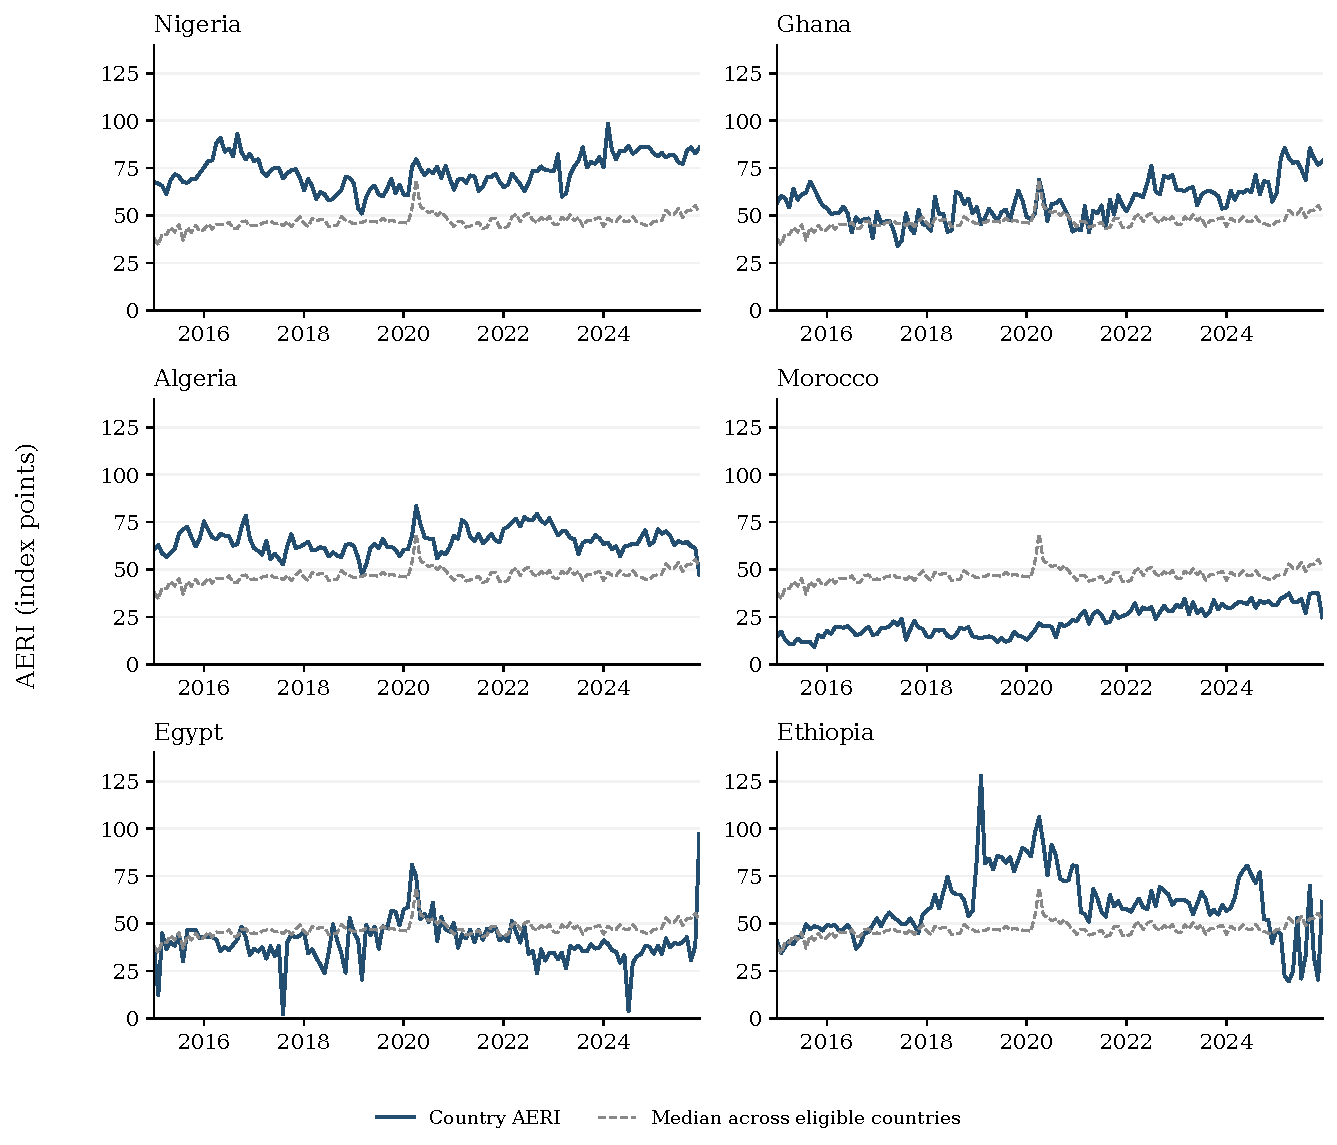
\includegraphics[width=.96\textwidth,height=.72\textheight,keepaspectratio]{Supplement_Figure_S3.pdf}
\caption{Monthly country AERI: Nigeria, Ghana, Algeria, Morocco, Egypt and Ethiopia}
\begin{singlespace}\footnotesize\textit{Notes:} Solid lines show monthly AERI. The dashed line is the median across countries with at least 100 retained articles in the corresponding month. No smoothing or country-specific rebasing is applied.\end{singlespace}
\end{figure}

\begin{figure}[htbp]\centering
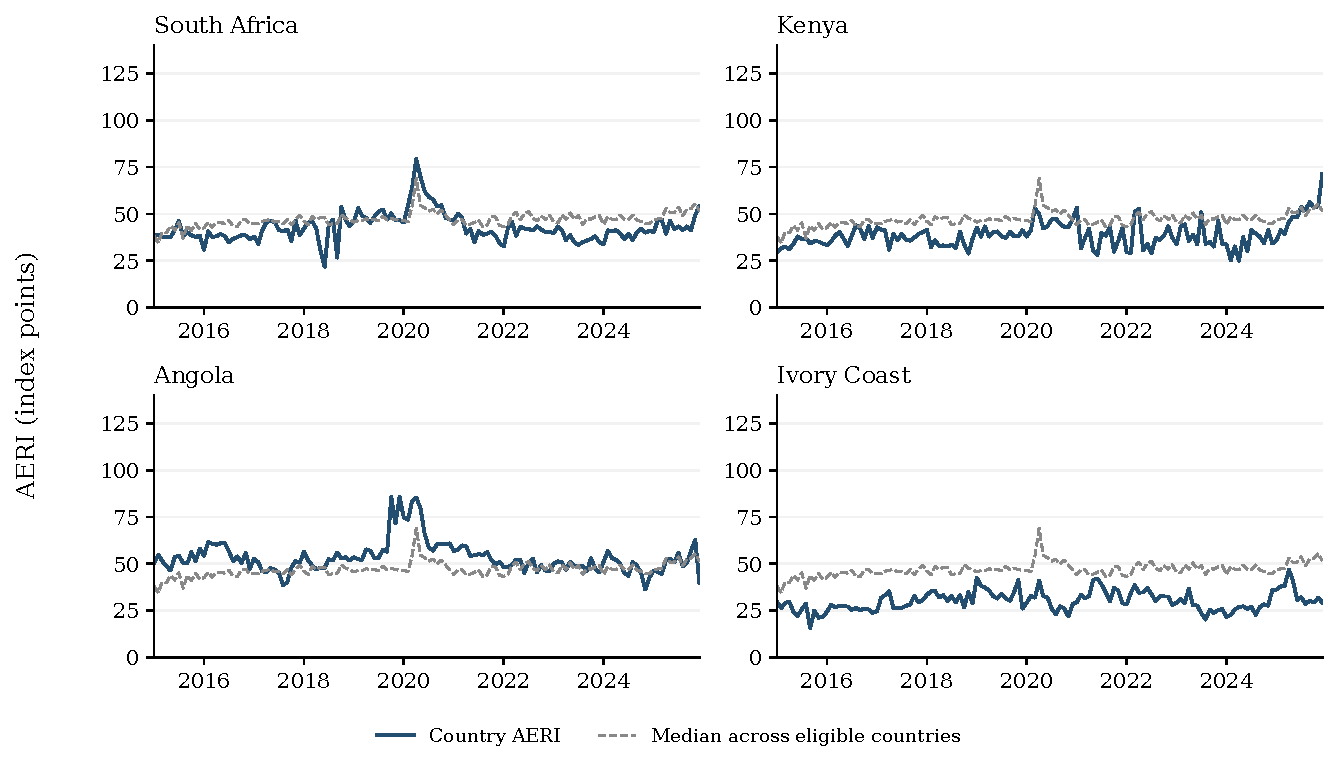
\includegraphics[width=.96\textwidth,height=.72\textheight,keepaspectratio]{Supplement_Figure_S4.pdf}
\caption{Monthly country AERI: South Africa, Kenya, Angola and Ivory Coast}
\begin{singlespace}\footnotesize\textit{Notes:} Definitions, timeline and vertical scale match the preceding figure. The reference median varies with the composition of eligible countries.\end{singlespace}
\end{figure}

\clearpage
\section*{References}
\addcontentsline{toc}{section}{References}
\begingroup\small\singlespacing
\printbibliography[heading=none]
\endgroup
\end{document}
